\section{Bundle Size}\label{sec:bundlesize}
%% FUNCTION: Shows that round robin is guaranteed to be EFX when every agent receives at most two
%% goods and all favourite goods differ, and that this guarantee breaks as soon as one agent
%% receives three goods. Since this break coincides with a change in divisibility, the section
%% leads to the next one.

We define "collision-freeness" as follows: All agents have different favorite goods. The collision rate $1-\#\{distinct favourite goods\}/n$. For $\rho = 1$ it equals to $1-1/n$. Collision-freeness does not occur there.

$\textit{Lemma}$: 

If the instance is collision-free, only Agent $i$ can envy Agent $j$, when $|A_j|>= 3$

Proof: Withtout collision, any agents receives their favourite good in the first round. When $A_j$ only has two goods, after eleminating one good the bundle only has one good left. And that good is not more valuable than his own favourite good. $m=< 2n$ ensures $|A_j| =< 2$

Implication: If the Instance is Collision free and $m=< 2n \Rightarrow RR-Allocation is EFX$

We checked this for every cell. 336 cells with $m=<2n$ and $\rho < 1$, all six $\theta$, 1.388.388 collision free instances, 0 exceptions.

The guarantee does not need an assumption about the distribution.

bitte die tabelle hierhin anteil collsionfree instances.

This condition gets rare quickly. From a ration of 0,749 for ( n =2, rho= 0) to 0,010 for (n=5, rho = 0,75) which only are 193 of 20000 instances.


\begin{figure}
    \centering
    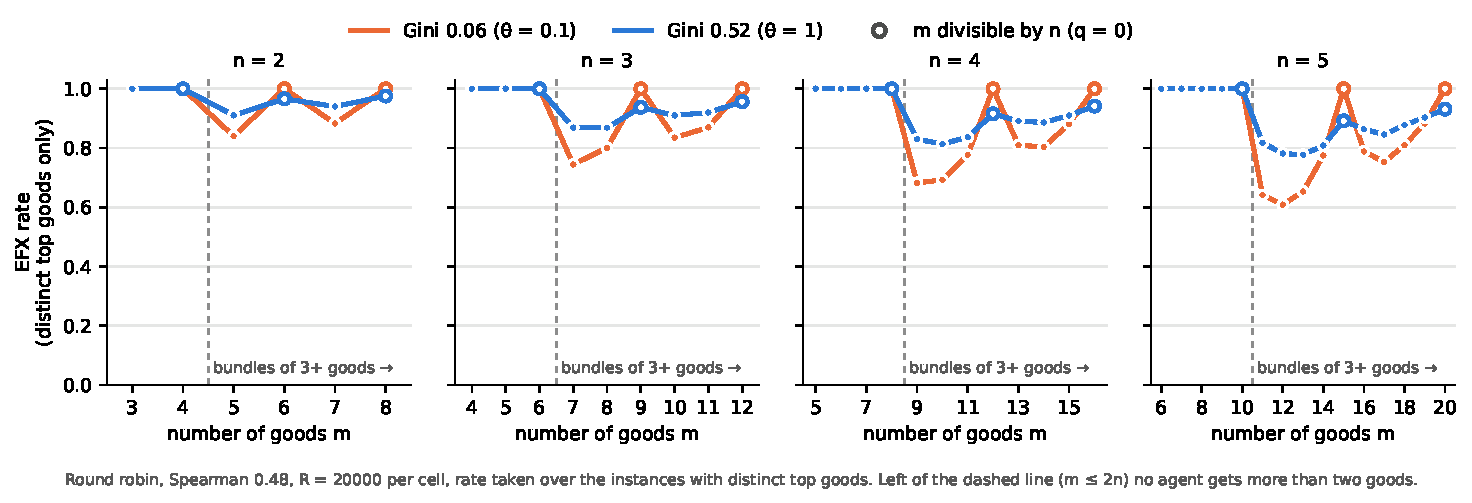
\includegraphics[width=1\linewidth]{block1_fig_break.pdf}
    \caption{Enter Caption}
    \label{fig:placeholder}
\end{figure}

For $n=4$, for $m=<8$ goods, meaning bundle size r=<2 we have a continous EFX Allocation through RR. At 9 goods, we conceive a efx bump to 0,830 (with gini 0,52) and 0,682 (at gini 0,06)
The EFX-quote under kollision free instances show a reocurring pattern that with the divisability of revover.

If we consider all instances however, those trends do not really show in the total graphic.

A bundle with two goods means for the EF1 EFX connection, lead $>=$ gap or "my bundle" $>=$ his best good. and thats secured by the own fav good. 
With three goods now its "my goods vs his two best goods" and the own fav good cannot secure both of them.
Thus, the only endangered pairs are "two vs three goods", for r=2 that are $(n-q) \cdot q$ pairs. 

With smaller $\theta$ is the EFX drop bigger, becaus the structurall lead of the pairs goes to null. 

We assume that the recovery after the drop bc of the growing lead.

Limitations, the depth of the drop also growths with $\rho$ ($n=5$: 0,942 bei $\rho=0$, 0,602 bei $\rho=0{,}75$). The graphic shows the case for $\rho = 0,75$

Another limitation is the assumption about the group we consider itself. in the real world, it rather unusual that everyone has their own favoutie good. It is rather decriptive and based on the quantitave model.

We also have to consider that the gap at 2n+1 can have two infuences.first that for the first time we have a bundle size of 3 but also the rest and divisability goes from 0 to 1. The drop could be the reslut of both changes, however you can split the two effects. becaus for smaller m<=2 there are also q>0  and the efx quote is still 1. The q alone does not break the EFX quote. But this only counts if we only consider the instances where there is collision freeness, considers for all instances this statement does not apply. 

Additionally our Lemma in independet from our distribution bc it only considers the values. If another valuation model creates values where each agents has a own favouite good, this Lemma also applies.

Our emperical foundings also allign with the scientific research, stating that Round Robin has dificouklties of finding ERX with q > 0 with cnstant proability. For an asymptotic case of our collision mechansims \cite{manurangsi2021}.

Also the EFX existance for m=<2n is proved. Moreover \cite{amanatidis2020multiple} prove that there exist and EFX alloctatin until m=<n+3






If every agent receives at most two goods and all favourite goods differ, use Round Robin: EFX is guaranteed, and both conditions can be checked in advance.“ Dazu: Die Bedingung wird mit mehr Personen und mehr Einigkeit schnell selten, und darüber hinaus bricht die Garantie.

How already consideres broadly. A central question is now how the drop behaves with other q's. 